\chapter{Mathematical Circuits Using Op.Amp.: Part I}


\section{Objectives}
\begin{itemize}
    \item To verify Op.Amp. circuits for basic amplification operations
    \item To verify Op.Amp. circuits for addition/substraction
\end{itemize}

\section{Materials}
\begin{itemize}
    \item Breadboard
    \item DC power supply
    \item Digital Multi-Meter
    \item Function Generator
    \item \hyperref[LM741_1]{Op.Amp. (LM741)}
    \item Oscilloscope
    \item Resistors
\end{itemize}

\section{Introduction}
    \subsection{Operational Amplifier}
        \begin{itemize}
            \item \textbf{What is the Operational Amplifier}\par
                Operational Amplifier, normal written as Op.Amp., are fundamental components in electronics which is used in analog electronics. It is constructed using a combination of several MOSFETs.\par
                Op.Amp. is a high-gain voltage amplifier with a differential input (negative and positive inputs).\par
                Operational amplifiers are versatile components that can be utilized in a variety of applications, including signal amplification, waveform oscillation, and performing mathematical operations.
        \end{itemize}
    \subsection{Specification}
        \begin{itemize}
            \item \hyperref[LM741_1]{Op.Amp. (LM741)}
        \end{itemize}
        
    \subsection{Circuit Diagram}
    \begin{figure}[h]

        \begin{subfigure}[h]{0.47\textwidth}
        \begin{center}
            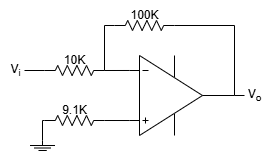
\includegraphics[width=1\linewidth]{Lab10/Lab10a.drawio.png}
            \caption{}
            \label{L10a}
        \end{center} 
        \end{subfigure}
    \hfill
    \vspace{0.2 cm}
        \begin{subfigure}[h]{0.47\textwidth}
        \begin{center}
            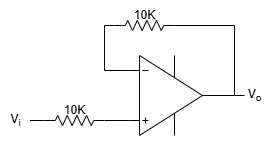
\includegraphics[width=1\linewidth]{Lab10/Lab10b.drawio.png}
            \caption{}
            \label{L10b}
        \end{center}
        \end{subfigure}
    \vfill
    
    \vspace{0.2 cm}
        \begin{subfigure}[h]{0.47\textwidth}
        \begin{center}
            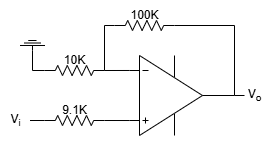
\includegraphics[width=1\linewidth]{Lab10/Lab10c.drawio.png} 
            \caption{}
            \label{L10c}
        \end{center}
        \end{subfigure}
    \hfill
        \begin{subfigure}[h]{0.47\textwidth}
        \begin{center}
            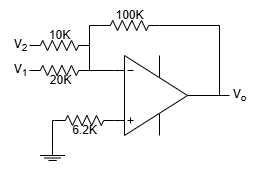
\includegraphics[width=1\linewidth]{Lab10/Lab10d.drawio.png}
            \caption{}
            \label{L10d}
        \end{center}
        \end{subfigure}

    \vspace{0.2 cm}
        \begin{subfigure}[h]{0.47\textwidth}
        \begin{center}
            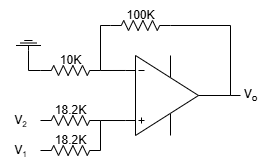
\includegraphics[width=1\linewidth]{Lab10/Lab10e.drawio.png}
            \caption{}
            \label{L10e}
        \end{center}
        \end{subfigure}
    \hfill
        \begin{subfigure}[h]{0.47\textwidth}
        \begin{center}
            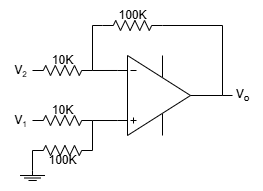
\includegraphics[width=1\linewidth]{Lab10/Lab10f.drawio.png}
            \caption{}
            \label{L10f}
        \end{center}
        \end{subfigure}
    \caption{Different fundamental Op.Amp. circuits}
    \label{l10figs}
    
    \end{figure}
    \FloatBarrier

\section{Detailed Procedures}
    \subsection{Analyzation}
    In this experiment, because it is not all the resistor's resistance can meet the requirement on the figures, some of the resistors are combined resistors, therefore for the accuracy all the components were measured, with the values of:
    \begin{itemize}
        \item 20K: 20.01K
        \item 10K: 9.775K
        \item 100K: 99.19K
        \item 6.2K: 6.218K
        \item 12K: 11.77K
        \item 18.2K: 18.0K\~18.11K
    \end{itemize}
    \begin{itemize}
        \item For Fig.\ref{L10a},
            \begin{equation}
                \begin{cases}
                    i=\frac{V_i}{10K}=\frac{-V_o}{100K}\\
                    V_o=-10V_i\\
                \end{cases}
            \end{equation}
        \item For Fig.\ref{L10b},
            \begin{equation}
                \begin{cases}
                    i=\frac{-V_o}{10K}\\
                    V_o=V_i\\
                \end{cases}
            \end{equation}
        \item For Fig.\ref{L10c},
            \begin{equation}
                \begin{cases}
                    i=\frac{-V_o}{100K}=\frac{V_i}{9.1K}\\
                    V_o=\frac{100V_i}{9.1}\\
                \end{cases}
            \end{equation}
        \item For Fig.\ref{L10d},
            \begin{equation}
                V_o=-5V_i-10V_2
            \end{equation}
        \item For Fig.\ref{L10e},
            \begin{equation}
                \begin{cases}
                    \frac{V_o10K}{10K+100K}=V_a\\
                    \frac{V_1-V_b}{18.2K}+\frac{V_2-V_b}{18.2K}=0\\
                    V_a=V_b\\
                    V_o=-\frac{11}{2}(V_1+V_2)\\
                \end{cases}
            \end{equation}
        \item For Fig.\ref{L10f},
            \begin{equation}
                \begin{cases}
                    \frac{100K}{10K+100K}\cdot(1+\frac{100K}{10K})\cdot V_1-\frac{100K}{10K}\cdot V_2=V_o\\
                    V_o=10V_1-10V_2\\
                \end{cases}
            \end{equation}
    \end{itemize}


    \subsection{Procedures}
    \begin{itemize}
        \item For Fig.\ref{L10a},
\begin{table}[h]
\centering
\begin{tabular}{|c|c|c|c|c|c|c|c|c|}
\hline
Vi & 0.1 & 0.3   & 0.5   & 0.7   & 0.9   & 1.1    & 1.3    & 1.5    \\ \hline
Vo & -1  & -3.05 & -5.09 & -7.11 & -9.16 & -11.15 & -11.36 & -11.36 \\ \hline
\end{tabular}
\end{table}
\FloatBarrier
        \item For Fig.\ref{L10b},
\begin{table}[h]
\centering
\begin{tabular}{|c|c|c|c|c|c|c|c|c|}
\hline
Vi & 0.1   & 0.3   & 0.5   & 0.7   & 0.9   & 1.1   & 1.3   & 1.5   \\ \hline
Vo & 0.091 & 0.299 & 0.499 & 0.695 & 0.896 & 1.096 & 1.296 & 1.498 \\ \hline
\end{tabular}
\end{table}
\FloatBarrier
        \item For Fig.\ref{L10c},
\begin{table}[h]
\centering
\begin{tabular}{|c|c|c|c|c|c|c|c|c|}
\hline
Vi & 0.1   & 0.3   & 0.5   & 0.7   & 0.9   & 1.1   & 1.3   & 1.5   \\ \hline
Vo & 0.091 & 0.299 & 0.499 & 0.695 & 0.896 & 1.096 & 1.296 & 1.498 \\ \hline
\end{tabular}
\end{table}
\FloatBarrier
        \item For Fig.\ref{L10d},
\begin{table}[h]
\centering
\begin{tabular}{|c|c|c|c|c|}
\hline
V1 & 0.1    & 0.5    & 0.1    & 1.0     \\ \hline
V2 & 0.2    & 0.1    & 0.5    & 0.4     \\ \hline
Vo & -2.053 & -5.580 & -3.516 & -11.362 \\ \hline
\end{tabular}
\end{table}
\FloatBarrier
        \item For Fig.\ref{L10e},
\begin{table}[h]
\centering
\begin{tabular}{|c|c|c|c|c|}
\hline
V1 & 0.1   & 0.5   & 0.8   & 1.0    \\ \hline
V2 & 0.2   & 0.3   & 0.5   & 1.0    \\ \hline
Vo & 1.640 & 4.439 & 7.205 & 10.638 \\ \hline
\end{tabular}
\end{table}
\FloatBarrier
        \item For Fig.\ref{L10f},
\begin{table}[h]
\centering
\begin{tabular}{|c|c|c|c|}
\hline
V1 & 0.1  & 0.5  & 1.0   \\ \hline
V2 & 0.4  & 0.1  & 0.4   \\ \hline
Vo & 4.79 & 5.57 & 10.65 \\ \hline
\end{tabular}
\end{table}
\FloatBarrier
    \end{itemize}
\FloatBarrier
    
\section{Discussion}
This experiment is conducting with using multiple combined resistors, this might cause the inaccuracy of the resistance.

\section{Conclusion}
In this experiment, we verified various operational amplifier circuits, these circuits present different functions. And these circuits performed expected results which very close to the results of theoretical relationship we predicted.\par
These circuits help me learn more about the operational amplifiers' practical usage in real life.\par
In summary, these experiments reinforce my theoretical concepts while emphasizing practical considerations. This knowledge is crucial for us about the concept of utilizing amplifiers in real-world applications.